\chapter{FFT Analyzer}
La \textbf{FFT} (Fast Fourier Transform) non è altro che un \textbf{algoritmo} che calcola più velocemente la \textbf{DFT} (Discrete Fourier Transform):
\begin{center}
    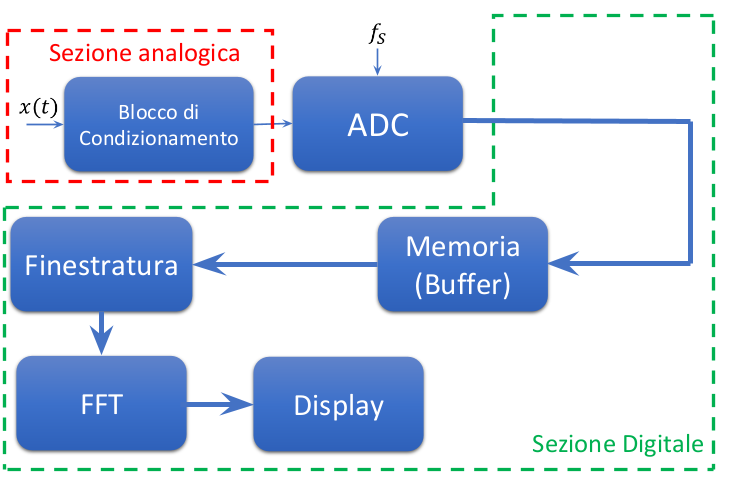
\includegraphics[width=\textwidth]{Images/figure30.png}
\end{center}
Il \textbf{segnale analogico} entra nel \textbf{blocco di condizionamento}, a valle del quale avremo la \textbf{conversione analogico digitale} che campiona il segnale ad una \textbf{frequenza di campionamento} $f_c$.\\
Il segnale viene poi immagazzinato in \textbf{memoria} e \textbf{finestrato}, e a questo punto viene effettuata la \textbf{FFT}.\\ \\
Vediamo i blocchi in dettaglio:\\
\begin{center}
    \textbf{Condizionamento}
\end{center}
Questo blocco ha lo scopo di \textbf{adattare il segnale analogico} per i blocchi che troverà a valle e opera la funzione di un \textbf{filtro} \textbf{passa basso}, con l'aggiunta della \textbf{protezione dal fenomeno di aliasing}.\\ \\
In particolare, il compito di questo filtro è quello di \textbf{limitare le componenti frequenziali} del segnale in ingresso, in modo tale da far si che la \textbf{massima frequenza }del segnale sia \textbf{minore della metà della frequenza di campionamento}.\\ \\
Entrando più nel dettaglio possiamo discernere \textbf{3 operazioni fondamentali}:
\begin{itemize}
    \item \textbf{Accoppiamento} (coupling)
    \item \textbf{Amplificatore}/\textbf{Attenuatore}
    \item \textbf{Anti-Aliasing}
\end{itemize}
\begin{center}
    \textbf{Memoria}
\end{center}
Identicamente alla \textbf{memoria dell'oscilloscopio}, anche la memoria dell' \textbf{FFT} viene gestita con la tecnica \textbf{FIFO}.\\ \\
\begin{center}
    \textbf{Finestratura}
\end{center}
Il calcolo della \textbf{FFT} si basa su \textbf{sequenze} di lunghezza N finite, mentre arrivano in continuazione campioni in uscita dall'A/D, quindi occorre selezionare dei blocchi di N campioni per volta.\\ \\
Questa operazione viene chiamata \textbf{finestratura} e consiste nel \textbf{moltiplicare} la sequenza di uscita per una \textbf{finestra} \textbf{rettangolare di lunghezza N}.\\ \\
Possiamo definire due tipi di campionamenti:
\begin{itemize}
    \item \textbf{Campionamento Sincrono}, in cui prendiamo un numero intero di periodi;
    \item \textbf{Campionamento Asincrono}, in cui non prendiamo un numero intero di periodi;
\end{itemize}
Nel caso di \textbf{campionamento asincrono}, si genereranno delle \textbf{discontinuità} che faranno nascere delle \textbf{componenti spettrali} non presenti nel segnale originario (\textbf{Spectral} \textbf{Leakage}).\\ \\
Proprio per questo esistono diverse tipologie di finestre:
\begin{itemize}
    \item \textbf{Rettangolare}
    \item \textbf{Hamming}
    \item \textbf{Blackman-Harris}
    \item \textbf{Flat Top}
\end{itemize}
\begin{center}
    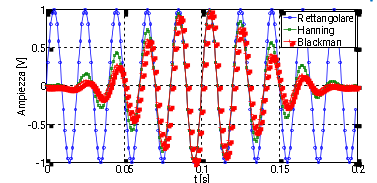
\includegraphics[width=.8\textwidth]{Images/figure47.png}
\end{center}